\documentclass[border=10pt]{standalone}
\usepackage{tikz}
\usepackage{amsmath}

\begin{document}
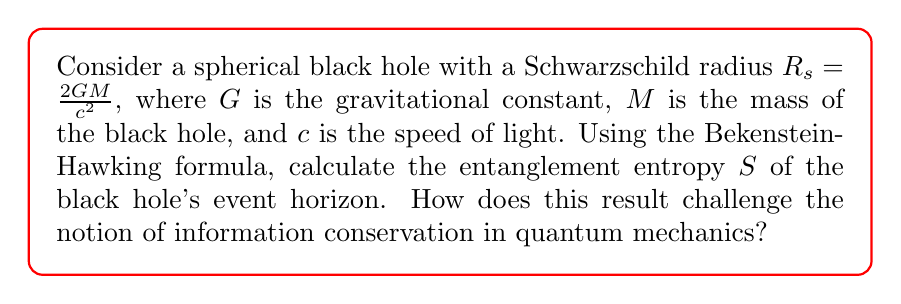
\begin{tikzpicture}
  \begin{scope}[
    every node/.style={font=\sansdefault},
    ]
    \node[
      draw=red,
      thick,
      rounded corners=5pt,
      inner sep=10pt,
      text width=10cm,
      align=justify,
      ] (text_box) at (0,0) {
Consider a spherical black hole with a Schwarzschild radius $R_s = \frac{2GM}{c^2}$, where $G$ is the gravitational constant, $M$ is the mass of the black hole, and $c$ is the speed of light. Using the Bekenstein-Hawking formula, calculate the entanglement entropy $S$ of the black hole's event horizon. How does this result challenge the notion of information conservation in quantum mechanics?
    };
  \end{scope}
\end{tikzpicture}
\end{document}